\documentclass[journal]{IEEEtran}
\usepackage{amsmath,amssymb}
\usepackage{graphicx}
\usepackage{booktabs}
\usepackage{multirow}
\usepackage{xcolor}
\usepackage{tikz}
\usetikzlibrary{arrows.meta,positioning,fit,calc}
\usepackage[hidelinks]{hyperref}
\usepackage{cite}

\newcommand{\todo}[1]{\textcolor{red}{[#1]}}

\begin{document}

\title{Learned Candidate Verification with a Promptable 3D Foundation Model for Fully Automatic Breast Tumour Segmentation in DCE-MRI}

\author{Bharath~Kumar~Vemuri,~\todo{Co-authors / Supervisor}%
\thanks{B.~K.~Vemuri is with the School of Data Science, Indian Institute of Science Education and Research (IISER) Thiruvananthapuram, India.}%
\thanks{\textcolor{red}{DRAFT, 13 October 2026. Results reflect experiments completed to date; the frequency-council stage (Section~V-C) is ongoing. References marked for verification before submission.}}}

\markboth{IEEE Journal of Biomedical and Health Informatics --- Draft}{Vemuri \MakeLowercase{\textit{et al.}}: Learned Candidate Verification for Breast DCE-MRI Segmentation}

\maketitle

\begin{abstract}
Automatic segmentation of the primary tumour in breast dynamic contrast-enhanced MRI (DCE-MRI) is hampered less by boundary errors than by false-positive enhancement: vessels, lymph nodes and background parenchymal enhancement that a voxel-wise network labels as tumour. Promptable foundation models such as SAM-Med3D segment accurately when given a good prompt but cannot be used without one. We propose a fully automatic finder--checker pipeline in which a 3D segmentation network (SegResNet) proposes connected-component candidates, a parameter-efficiently adapted SAM-Med3D-turbo examines each candidate from a box prompt, and a \emph{learned candidate verifier} decides which candidates form the final mask. The checker is trained with realistic, perturbed and negative box prompts so that it can respond to imperfect, automatically generated prompts. The verifier is a gradient-boosted classifier over 11 descriptors of candidate geometry, finder confidence and checker response, trained on candidates from the training set and calibrated on a held-out validation set. On the 306-case official test set of the multi-centre MAMA-MIA dataset, learned verification improves the mean Dice from 0.684 (segmentation network with connected-component filtering) and 0.699 (rule-based agreement filtering) to 0.735 ($p<10^{-3}$), reduces the median 95th-percentile Hausdorff distance from 7.3 to 3.6~mm and raises the normalised surface Dice from 0.716 to 0.783. The verifier separates true from false candidates with an AUC of 0.916, higher than any single cue. In contrast, fine-tuning the checker to reject the finder's false positives traded sensitivity for specificity without improving discrimination, indicating that the frozen foundation model already encodes the necessary evidence and that a learned decision layer exploits it more effectively.
\end{abstract}

\begin{IEEEkeywords}
Breast cancer, DCE-MRI, tumour segmentation, foundation models, SAM-Med3D, false-positive reduction, candidate verification, gradient boosting.
\end{IEEEkeywords}

\section{Introduction}
\IEEEPARstart{D}{ynamic} contrast-enhanced MRI (DCE-MRI) is the most sensitive imaging modality for breast cancer and is routinely used for staging and for monitoring response to neoadjuvant chemotherapy. Volumetric delineation of the primary tumour underpins quantitative tumour-size and response measurements and radiomics, but manual 3D annotation is time-consuming and variable. Automatic 3D segmentation is therefore of direct clinical interest.

Convolutional encoder--decoder networks such as nnU-Net~\cite{isensee2021nnunet} and SegResNet~\cite{myronenko2019segresnet} achieve good overlap on many 3D tasks, yet in breast DCE-MRI a characteristic failure mode dominates: structures that enhance after contrast administration---blood vessels, axillary lymph nodes, benign lesions and background parenchymal enhancement---are labelled as tumour. In the multi-centre MAMA-MIA dataset~\cite{garrucho2025mamamia}, 66\% of the official test examinations contain at least one such false-positive connected component in the output of a strong SegResNet baseline. Because the Dice coefficient penalises every false-positive voxel, deciding \emph{which} predicted regions to keep is as important as refining their boundaries.

Promptable segmentation foundation models, beginning with the Segment Anything Model (SAM)~\cite{kirillov2023sam} and its medical and volumetric descendants~\cite{ma2024medsam,wang2023sammed3d}, segment a target accurately when given a box or click prompt. They are, however, not automatic: someone has to supply the prompt. Fine-tuned on MAMA-MIA with ground-truth boxes, SAM-Med3D-turbo reaches a Dice of 0.708 on the test set in our experiments---higher than the fully automatic SegResNet (0.684)---but this oracle setting is unavailable in practice.

We combine the two model families in a \emph{finder--checker} design. The finder (SegResNet) localises candidate regions without prompts; the checker (SAM-Med3D-turbo, adapted with low-rank adapters) examines each candidate from an automatically derived box prompt. The central question is how to turn the finder's and checker's outputs into a final decision. Hand-crafted rules, such as keeping candidates on which both models agree, use a single cue with an arbitrary threshold. We instead learn the decision from data.

Our contributions are:
\begin{enumerate}
\item A fully automatic finder--checker pipeline for 3D breast tumour segmentation in which a promptable 3D foundation model is prompted by connected-component candidates of a segmentation network, with the checker trained on realistic, perturbed and negative box prompts so that it tolerates imperfect automatic prompts and can answer ``no tumour here''.
\item A \emph{learned candidate verifier}: a gradient-boosted classifier over 11 descriptors of candidate geometry, finder confidence and checker response that improves the test Dice from 0.684/0.699 to 0.735, with consistent gains in boundary metrics and statistical significance, and an exact, mask-free procedure for selecting its operating point.
\item An analysis showing that the frozen checker already discriminates true from false candidates (AUC 0.82 from its soft predicted volume alone), whereas fine-tuning it on the finder's false positives reduces sensitivity without improving discrimination---evidence that, for foundation-model checkers, a learned decision layer is more effective than further adaptation of the checker.
\end{enumerate}

\section{Related Work}
\subsection{3D segmentation networks}
nnU-Net~\cite{isensee2021nnunet} established a strong self-configuring baseline for 3D medical segmentation; SegResNet~\cite{myronenko2019segresnet}, an encoder--decoder with residual blocks, is a widely used and efficient alternative available in MONAI~\cite{cardoso2022monai}. Both are trained voxel-wise and are therefore prone to false positives on structures whose appearance resembles the target, a problem typically addressed with connected-component post-processing.

\subsection{Promptable foundation models}
SAM~\cite{kirillov2023sam} introduced promptable segmentation at scale; MedSAM~\cite{ma2024medsam} adapted it to medical images, and SAM-Med3D~\cite{wang2023sammed3d} extended the architecture to volumetric data with 3D prompts. Parameter-efficient fine-tuning such as low-rank adaptation (LoRA)~\cite{hu2022lora} allows these models to be specialised with few trainable parameters. Their reliance on prompts motivates pipelines in which prompts are generated automatically; the reliability of such pipelines then depends on how imperfect automatic prompts and false candidates are handled, which is the focus of this work.

\subsection{Breast DCE-MRI segmentation}
MAMA-MIA~\cite{garrucho2025mamamia} provides 1,506 expert-segmented DCE-MRI examinations from four collections (DUKE, ISPY1, ISPY2, NACT) with an official train/test split, enabling a multi-centre evaluation. The heterogeneity of scanners and protocols across collections makes false-positive enhancement and domain shift central difficulties.

\section{Methods}

\begin{figure*}[t]
\centering
\resizebox{\textwidth}{!}{%
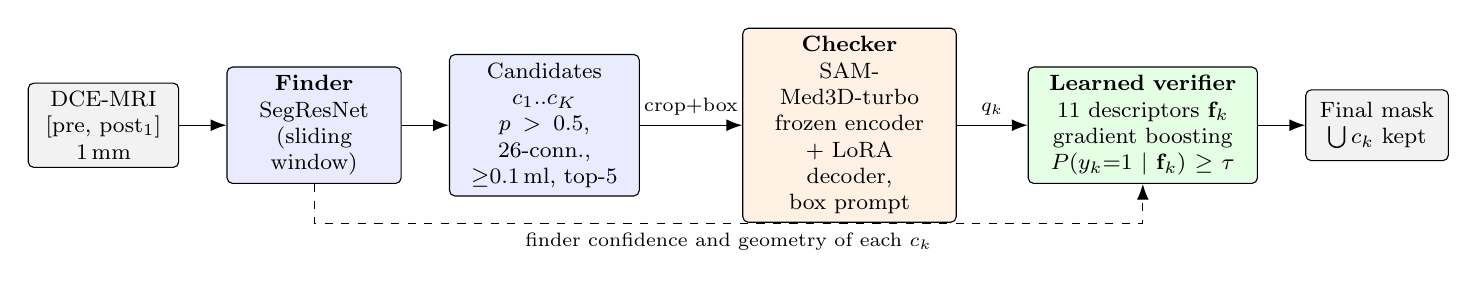
\begin{tikzpicture}[
  font=\footnotesize, >={Latex[length=2mm]},
  box/.style={draw, rounded corners=2pt, align=center, minimum height=9mm, inner sep=3pt, fill=#1},
  box/.default=white]
\node[box=gray!10, text width=17mm] (mri) {DCE-MRI\\{[pre, post$_1$]}\\1\,mm};
\node[box=blue!8, text width=20mm, right=6mm of mri] (finder) {\textbf{Finder}\\SegResNet\\(sliding window)};
\node[box=blue!8, text width=22mm, right=6mm of finder] (cand) {Candidates $c_1..c_K$\\$p>0.5$, 26-conn.,\\$\ge$0.1\,ml, top-5};
\node[box=orange!10, text width=25mm, right=13mm of cand] (checker) {\textbf{Checker}\\SAM-Med3D-turbo\\frozen encoder + LoRA\\decoder, box prompt};
\node[box=green!10, text width=27mm, right=9mm of checker] (verifier) {\textbf{Learned verifier}\\11 descriptors $\mathbf{f}_k$\\gradient boosting\\$P(y_k{=}1\mid\mathbf{f}_k)\ge\tau$};
\node[box=gray!10, text width=16mm, right=6mm of verifier] (out) {Final mask\\$\bigcup c_k$ kept};
\draw[->] (mri) -- (finder);
\draw[->] (finder) -- (cand);
\draw[->] (cand) -- node[above, font=\scriptsize]{crop+box} (checker);
\draw[->] (checker) -- node[above, font=\scriptsize]{$q_k$} (verifier);
\draw[->] (verifier) -- (out);
\draw[->, dashed] (finder.south) -- ++(0,-5mm) -| node[pos=0.25, below, font=\scriptsize]{finder confidence and geometry of each $c_k$} (verifier.south);
\end{tikzpicture}}
\caption{Fully automatic finder--checker pipeline with learned candidate verification. The finder proposes connected-component candidates; the checker segments each candidate from an automatically derived box prompt; the verifier combines geometry, finder confidence and checker response to decide which candidates form the final mask. No ground truth or human prompt is used at inference.}
\label{fig:pipeline}
\end{figure*}

\subsection{Data and preprocessing}
We use all 1,506 examinations of MAMA-MIA~\cite{garrucho2025mamamia}. The 306 cases of the official test set are used only for final evaluation; the remaining 1,200 are split into 1,080 training and 120 validation cases with a fixed seed (stratified by collection). Each examination is represented by the pre-contrast and first post-contrast phases, reoriented to RAS, resampled to 1\,mm isotropic spacing and scaled per channel to $[0,1]$ using the 1st and 99th percentiles. Labels mark the primary tumour only.

\subsection{Finder: SegResNet}
The finder is a 3D SegResNet~\cite{myronenko2019segresnet} (16 initial filters, encoder blocks $(1,2,2,4)$, decoder blocks $(1,1,1)$) with three input channels: pre-contrast, post-contrast and their difference. It is trained on random $96^3$ patches (four per patient per epoch, sampled around the tumour or at random body locations) with a combined Dice and cross-entropy loss, AdamW (learning rate $2\times10^{-4}$, weight decay $10^{-5}$), a cosine schedule with three warm-up epochs and mixed precision. After 60 epochs, training was extended to 100 epochs with a warm-restart cycle (peak learning rate $10^{-4}$, two warm-up epochs). The checkpoint with the highest validation Dice is used. Inference uses Gaussian-weighted sliding windows ($96^3$, overlap 0.5). As the finder-only baseline, connected components smaller than 20\% of the largest component are removed (\emph{rel20}; chosen on validation among several rules).

\subsection{Checker: SAM-Med3D-turbo with box prompts}
The checker is SAM-Med3D-turbo~\cite{wang2023sammed3d}. Following its pre-processing, inputs are $128^3$ crops of the post-contrast phase at 1.5\,mm, z-normalised over foreground voxels. The image encoder is frozen; its embeddings ($384\times8^3$) are pre-computed for one tumour-centred and three randomly shifted crops ($\pm$24\,mm) per training case. The mask decoder is adapted with LoRA~\cite{hu2022lora} (rank 8, $\alpha=16$) on its query and value projections, and two learnable corner tokens encode 3D box prompts; in total 71,424 parameters are trained. Each training step uses either a box prompt (probability 0.5) or a random click, followed by up to four corrective clicks with the previous low-resolution mask fed back; the loss is binary cross-entropy plus soft Dice on the upsampled logits (AdamW, learning rate $5\times10^{-4}$, batch size 8).

To make the checker robust to automatic prompts, box prompts are drawn from three types: \emph{clean} (ground-truth box $\pm5$ voxels, 40\%), \emph{messy} (scaled by 0.7--1.8 and shifted by up to 40\% of the tumour size, 40\%) and \emph{negative} (placed on tumour-free tissue with an empty target, 20\%). The validation criterion is the mean of clean-box Dice, messy-box Dice and the rejection rate on negative boxes (prediction below 0.1\,ml). We refer to this checker as \emph{S2b}; a variant trained with clean boxes only is \emph{S2a}. The checker is trained for 100 epochs.

\subsection{Candidate generation and checker response}
Let $p(\mathbf{x})$ be the finder probability. The binary map $p>0.5$ is decomposed into 26-connected components; components smaller than 0.1\,ml are discarded and the $K=5$ largest are kept as candidates $c_1,\dots,c_K$. For each candidate, a checker crop is centred on the bounding box of $c_k$ and the bounding box itself is the prompt. The checker returns a probability map $q_k$ over the crop, which is pasted back and resampled to the 1\,mm grid.

\subsection{Learned candidate verification}
Each candidate is described by an 11-dimensional vector $\mathbf{f}_k$ grouped as follows.
\emph{Geometry}: log volume, volume relative to the largest candidate, an indicator of the largest candidate, size rank and the number of candidates.
\emph{Finder confidence}: mean and maximum of $p$ within $c_k$.
\emph{Checker response}: agreement $\mathrm{Dice}(q_k>0.5,\,c_k)$, hard volume $|q_k>0.5|$, soft volume $\sum q_k$, and the log ratio of soft volume to candidate volume.
All descriptors are computed without ground truth.

A training label $y_k=1$ is assigned if $c_k$ overlaps the reference tumour mask. Applying the pipeline to the 1,080 training cases produced 2,561 candidates (1,246 positive, 1,315 negative). We fit an $\ell_2$-regularised logistic regression on standardised descriptors and a histogram-based gradient-boosted tree ensemble~\cite{friedman2001gbm,pedregosa2011sklearn} (300 trees, depth 3, learning rate 0.05, $\ell_2$ penalty 1.0), both with class-balanced weights. At inference the final mask is
\begin{equation}
\hat{M}=\bigcup_{k:\,\hat{P}(y_k=1\mid\mathbf{f}_k)\ge\tau} c_k ,
\end{equation}
and if no candidate reaches $\tau$ the most probable candidate is kept, since every examination contains a tumour. The classifier and $\tau\in\{0.05,0.10,\dots,0.95\}$ are chosen jointly by mean Dice on the validation set; the test set is evaluated once.

Because candidates are disjoint, the Dice of any selection $S$ follows exactly from per-candidate statistics,
\begin{equation}
\mathrm{Dice}(S)=\frac{2\sum_{k\in S}|c_k\cap G|}{\sum_{k\in S}|c_k|+|G|},
\end{equation}
with $G$ the reference mask, so the full classifier $\times$ threshold grid is evaluated without storing volumetric predictions.

\subsection{Comparison: retraining the checker on hard negatives}
As an alternative to learned verification, we fine-tuned the S2b checker so that it rejects the finder's false positives directly. Candidates were mined from the training cases with the same crop and box as the pipeline (finder threshold 0.3, top 8 to increase the number of negatives), yielding 3,274 candidates of which 2,033 were false. Batches of real false candidates (target: empty mask) and real true candidates (target: tumour) were mixed into the S2b training scheme. Two settings were evaluated: (i) 25\%/10\% false/true batches, learning rate $2\times10^{-4}$; (ii) balanced 20\%/20\% batches, learning rate $5\times10^{-5}$, with model selection restricted to epochs that retain at least 95\% of true candidates on validation.

\subsection{Evaluation}
We report the Dice coefficient, the 95th-percentile Hausdorff distance (HD95, median over cases because of its skewed distribution), the normalised surface Dice at 2\,mm tolerance (NSD)~\cite{nikolov2021nsd} and the number of missed tumours (Dice $<0.1$), all at 1\,mm resolution on the full volume. Candidate discrimination is measured by the area under the ROC curve (AUC) for true versus false candidates. Paired comparisons use the two-sided Wilcoxon signed-rank test~\cite{wilcoxon1945} on per-case Dice. Unless stated otherwise, results are on the 306-case official test set.

\section{Results}

\subsection{Finder and checker in isolation}
Table~\ref{tab:finder} summarises the finder. Extending training from 60 to 100 epochs improved the rel20 Dice from 0.655 to 0.684 and halved the median HD95. Conditioning the finder on clinical text prompts through feature-wise modulation (an earlier variant) gave no improvement (0.650 vs.\ 0.655, $p=0.94$) and was not pursued.

\begin{table}[t]
\centering
\caption{Finder (SegResNet) on the test set, after rel20 filtering.}
\label{tab:finder}
\setlength{\tabcolsep}{4pt}
\begin{tabular}{lccccc}
\toprule
Model & Dice (raw) & Dice & HD95 (mm) & NSD & Missed \\
\midrule
SegResNet, 60 ep. & 0.640 & 0.655 & 16.0 & 0.681 & 15 \\
SegResNet, 100 ep. & 0.671 & \textbf{0.684} & \textbf{7.3} & \textbf{0.716} & 14 \\
\bottomrule
\end{tabular}
\end{table}

Table~\ref{tab:checker} reports the checker with prompts derived from the ground truth (oracle prompts), which bounds what the checker can contribute. Fine-tuning raised the single-box Dice of SAM-Med3D-turbo to 0.708. Training with messy and negative boxes (S2b) cost 0.01 Dice on clean boxes but enabled rejection of 96.7\% of synthetic negative boxes.

\begin{table}[t]
\centering
\caption{Checker with oracle prompts on the test set (full resolution). Not fully automatic; shown as an upper reference.}
\label{tab:checker}
\setlength{\tabcolsep}{4pt}
\begin{tabular}{llccc}
\toprule
Checker & Prompt & Dice & HD95 (mm) & NSD \\
\midrule
Zero-shot & 1 click & 0.520 & 9.0 & 0.439 \\
Zero-shot & 5 clicks & 0.618 & 6.0 & 0.576 \\
S2a (clean boxes) & 1 click & 0.650 & 5.9 & 0.644 \\
S2a (clean boxes) & box & 0.708 & 4.4 & 0.729 \\
S2a (clean boxes) & 5 clicks & 0.717 & 4.6 & 0.738 \\
S2b (realistic boxes) & box & 0.698 & -- & -- \\
S2b (realistic boxes) & messy box & 0.653 & -- & -- \\
\bottomrule
\end{tabular}
\end{table}

\subsection{Fully automatic pipeline}
The finder produced candidates on false-positive enhancement in 66\% of test cases (836 candidates: 349 true, 487 false; median volume 9.2\,ml for true and 0.85\,ml for false candidates). Table~\ref{tab:main} compares decision strategies. A rule keeping candidates with checker agreement $\ge0.7$ (rule-based jury) improved Dice and HD95 over the finder but increased the number of missed tumours from 14 to 26, because it discarded true candidates on which the checker only partially agreed. The learned verifier, which selected gradient boosting with $\tau=0.60$ on validation, reached a test Dice of 0.735, significantly higher than both the finder ($p=7\times10^{-8}$) and the rule-based jury ($p=8\times10^{-4}$), with the lowest HD95 (3.6\,mm), the highest NSD (0.783) and fewer misses than the rule. Per case, the verifier improved the Dice by more than 0.05 over the rule-based jury in 39 cases and decreased it in 14. Selecting candidates perfectly would give 0.787, leaving a gap of 0.05.

\begin{table}[t]
\centering
\caption{Fully automatic segmentation on the test set (306 cases) and validation Dice (120 cases). Oracle: all candidates that touch the tumour are kept.}
\label{tab:main}
\setlength{\tabcolsep}{3pt}
\resizebox{\columnwidth}{!}{%
\begin{tabular}{lcccccc}
\toprule
Method & Val & Test & SD & HD95 & NSD & Missed \\
\midrule
Finder + rel20 & 0.724 & 0.684 & 0.243 & 7.3 & 0.716 & 14 \\
Finder + checker, rules (S2a)$^\dagger$ & -- & 0.675 & -- & -- & -- & -- \\
Finder + checker, rule-based jury & 0.747 & 0.699 & 0.280 & 4.1 & 0.744 & 26 \\
\textbf{Finder + checker, learned verifier} & \textbf{0.766} & \textbf{0.735} & 0.243 & \textbf{3.6} & \textbf{0.783} & 17 \\
\midrule
Oracle candidate selection & 0.812 & 0.787 & -- & -- & -- & -- \\
\bottomrule
\multicolumn{7}{l}{\scriptsize $^\dagger$Earlier configuration with the 60-epoch finder and the S2a checker.}
\end{tabular}}
\end{table}

Table~\ref{tab:coll} breaks the results down by collection. The largest gain occurred on DUKE (0.544 $\rightarrow$ 0.674), the collection with the most false-positive enhancement (72\% of its training candidates were false). On ISPY2 the verifier improved Dice by 0.04. On the small NACT subset (17 cases) the mean decreased; this was caused by three cases in which the verifier preferred a false candidate over the true one, while the remaining 14 cases were unchanged.

\begin{table}[t]
\centering
\caption{Test Dice per collection.}
\label{tab:coll}
\setlength{\tabcolsep}{3pt}
\begin{tabular}{lcccc}
\toprule
Collection ($n$) & Finder + rel20 & Rule-based jury & Learned verifier \\
\midrule
DUKE (91) & 0.544 & 0.587 & \textbf{0.674} \\
ISPY1 (67) & 0.729 & \textbf{0.743} & 0.733 \\
ISPY2 (131) & 0.753 & 0.752 & \textbf{0.793} \\
NACT (17) & \textbf{0.720} & 0.719 & 0.626 \\
\bottomrule
\end{tabular}
\end{table}

\subsection{Candidate discrimination}
Table~\ref{tab:auc} lists the AUC of individual descriptors and of the learned verifier for separating true from false candidates. The checker's soft volume alone reached 0.80--0.82, confirming that the checker responds differently to tumours and to false enhancement even though it was never trained on the finder's false positives. Combining all descriptors raised the AUC to 0.903 on validation and 0.916 on test.

\begin{table}[t]
\centering
\caption{AUC for true vs.\ false candidates.}
\label{tab:auc}
\setlength{\tabcolsep}{5pt}
\begin{tabular}{lcc}
\toprule
Score & Validation & Test \\
\midrule
Checker soft volume & 0.801 & 0.822 \\
Checker agreement & 0.844 & -- \\
Finder mean probability & 0.866 & -- \\
Logistic regression (11 descriptors) & 0.898 & -- \\
\textbf{Gradient boosting (11 descriptors)} & \textbf{0.903} & \textbf{0.916} \\
\bottomrule
\end{tabular}
\end{table}

\subsection{Robustness of the operating point}
The threshold was selected on validation ($\tau=0.60$). The best threshold in hindsight on the test set ($\tau=0.75$) would give 0.741, only 0.006 more, indicating that the selection did not overfit the validation set. Test cases more often had no candidate above $\tau$ (27 cases, 9\%) than validation cases (5 cases, 4\%), reflecting a harder test distribution; replacing the most-probable fallback by the largest candidate lowered the validation Dice (0.759) and was therefore not adopted.

\subsection{Retraining the checker on hard negatives}
Table~\ref{tab:s2c} contrasts learned verification with retraining the checker. With imbalanced batches, the checker learned to reject 84\% of the finder's false candidates but also rejected 35\% of true tumours, and its Dice on true candidates fell from 0.595 to 0.419. With balanced batches and a constraint of retaining at least 95\% of true candidates, no epoch satisfied the constraint while rejecting more false candidates; the trade-off was governed by a shift of the operating point, and the validation AUC decreased from 0.801 to 0.77--0.80. The model selected under the constraint was therefore identical to S2b.

\begin{table}[t]
\centering
\caption{Retraining the checker on the finder's false positives (test candidates; rejection: prediction $<0.1$\,ml).}
\label{tab:s2c}
\setlength{\tabcolsep}{3pt}
\begin{tabular}{lcccc}
\toprule
Checker & False rejected & True kept & Dice (true) & AUC \\
\midrule
S2b (no hard negatives) & 0.6\% & 99.7\% & 0.595 & 0.822 \\
+ hard negatives, imbalanced & 84.4\% & 65.0\% & 0.419 & -- \\
+ hard negatives, balanced$^\ddagger$ & 0.6\% & 99.7\% & 0.595 & 0.822 \\
\bottomrule
\end{tabular}

\vspace{1mm}
\parbox{\columnwidth}{\scriptsize $^\ddagger$No epoch kept $\ge$95\% of true candidates on validation while rejecting more false ones; the selected model equals S2b. Validation AUC fell from 0.80 to 0.77 during training.}
\end{table}

\section{Discussion}

\subsection{Why learned verification works}
The finder's errors in breast DCE-MRI are dominated by whole false components rather than imprecise boundaries, so a decision at the level of candidates addresses the main error mode directly. Each cue is informative but imperfect: size favours the tumour but fails on small lesions; finder confidence is high for strongly enhancing vessels; checker agreement penalises tumours that the checker segments more generously than the finder. A non-linear classifier can exploit interactions---for example, a large, confidently detected candidate is retained even when agreement is moderate---which explains why the combination (AUC 0.92) outperforms every single cue (0.80--0.87) and why the learned rule recovers tumours that the agreement rule discarded (17 vs.\ 26 misses).

\subsection{Adapting the checker versus learning the decision}
The hard-negative experiments indicate that the frozen checker already encodes the relevant evidence: its soft volume separates true from false candidates with AUC 0.82 without ever seeing the finder's false positives, yet additional supervision on those false positives did not increase separability and degraded segmentation. Teaching a mask decoder to output empty masks shifts its overall calibration rather than sharpening its discrimination. Placing the decision in a separate, lightweight layer leaves the checker's segmentation untouched and is cheap to train (seconds on a CPU).

\subsection{Limitations and ongoing work}
Results are from a single split and a single training seed; confidence intervals across seeds and leave-one-collection-out evaluation are in progress. The verifier is trained on candidates from cases the finder was trained on, where the finder is more confident than on unseen cases; cross-fitted verification probabilities (training AUC 0.93 vs.\ 0.97 in-sample, test 0.92) mitigate this when the verifier's output is used for further learning. Performance decreased on the small NACT subset, and 15 of the 17 remaining misses had a true candidate available, indicating room for descriptors that compare candidates within a case. The verifier keeps or removes whole finder components and cannot correct boundaries.

To address the latter, we are developing a \emph{frequency council}: four independent experts operating on groups of 3D Haar wavelet sub-bands~\cite{mallat1989wavelet} (low-pass shape, one-axis edges, two-axis corners and high-pass texture), each receiving the image together with the finder map and the verifier-weighted checker map, combined by a voxel-wise gate and trained with dual supervision from the reference masks and from regions where finder and checker agree. A complementary frequency adapter injects wavelet sub-band information into the frozen checker's embedding through a zero-initialised residual branch with learned per-band weights. In a further step, acquisition geometry (slice thickness, in-plane spacing, field strength) will condition the band weights, testing whether acquisition metadata can guide frequency selection across scanners. These components are implemented and under evaluation; their results will be reported against the learned-verification baseline established here (Dice 0.735).

\section{Conclusion}
For fully automatic breast tumour segmentation in DCE-MRI, combining a segmentation network with a promptable 3D foundation model is effective when the decision about which candidate regions to keep is learned rather than hand-crafted. A gradient-boosted verifier over geometry, finder confidence and checker response raised the test Dice on MAMA-MIA from 0.684 to 0.735 and improved boundary metrics consistently, whereas adapting the checker itself to the finder's false positives did not improve discrimination. Learned verification provides a strong, interpretable and inexpensive baseline on which frequency-aware and acquisition-aware refinements can build.

\section*{Acknowledgment}
\todo{Funding, compute (Kaggle GPUs), MAMA-MIA data providers.}

\begin{thebibliography}{99}
\bibitem{isensee2021nnunet}
F.~Isensee, P.~F.~Jaeger, S.~A.~A.~Kohl, J.~Petersen, and K.~H.~Maier-Hein, ``nnU-Net: A self-configuring method for deep learning-based biomedical image segmentation,'' \emph{Nature Methods}, vol.~18, pp.~203--211, 2021.

\bibitem{myronenko2019segresnet}
A.~Myronenko, ``3D MRI brain tumor segmentation using autoencoder regularization,'' in \emph{Brainlesion: Glioma, Multiple Sclerosis, Stroke and Traumatic Brain Injuries (BrainLes 2018)}, LNCS, vol.~11384, Springer, 2019, pp.~311--320.

\bibitem{garrucho2025mamamia}
L.~Garrucho \emph{et~al.}, ``A large-scale multicenter breast cancer DCE-MRI benchmark dataset with expert segmentations,'' \emph{Scientific Data}, 2025. \todo{verify volume/article number}

\bibitem{kirillov2023sam}
A.~Kirillov \emph{et~al.}, ``Segment anything,'' in \emph{Proc. IEEE/CVF Int. Conf. Comput. Vis. (ICCV)}, 2023, pp.~4015--4026.

\bibitem{ma2024medsam}
J.~Ma, Y.~He, F.~Li, L.~Han, C.~You, and B.~Wang, ``Segment anything in medical images,'' \emph{Nature Communications}, vol.~15, art.~654, 2024.

\bibitem{wang2023sammed3d}
H.~Wang \emph{et~al.}, ``SAM-Med3D: Towards general-purpose segmentation models for volumetric medical images,'' arXiv:2310.15161, 2023.

\bibitem{hu2022lora}
E.~J.~Hu \emph{et~al.}, ``LoRA: Low-rank adaptation of large language models,'' in \emph{Proc. Int. Conf. Learn. Represent. (ICLR)}, 2022.

\bibitem{cardoso2022monai}
M.~J.~Cardoso \emph{et~al.}, ``MONAI: An open-source framework for deep learning in healthcare,'' arXiv:2211.02701, 2022.

\bibitem{friedman2001gbm}
J.~H.~Friedman, ``Greedy function approximation: A gradient boosting machine,'' \emph{Ann. Statist.}, vol.~29, no.~5, pp.~1189--1232, 2001.

\bibitem{pedregosa2011sklearn}
F.~Pedregosa \emph{et~al.}, ``Scikit-learn: Machine learning in Python,'' \emph{J. Mach. Learn. Res.}, vol.~12, pp.~2825--2830, 2011.

\bibitem{nikolov2021nsd}
S.~Nikolov \emph{et~al.}, ``Clinically applicable segmentation of head and neck anatomy for radiotherapy: Deep learning algorithm development and validation study,'' \emph{J. Med. Internet Res.}, vol.~23, no.~7, e26151, 2021.

\bibitem{wilcoxon1945}
F.~Wilcoxon, ``Individual comparisons by ranking methods,'' \emph{Biometrics Bulletin}, vol.~1, no.~6, pp.~80--83, 1945.

\bibitem{mallat1989wavelet}
S.~G.~Mallat, ``A theory for multiresolution signal decomposition: The wavelet representation,'' \emph{IEEE Trans. Pattern Anal. Mach. Intell.}, vol.~11, no.~7, pp.~674--693, 1989.
\end{thebibliography}

\end{document}
